%=========================================================================
% fig-tuning-vectorization-convolution-access.tex
%=========================================================================

\begin{figure}[h!]

  \centering
  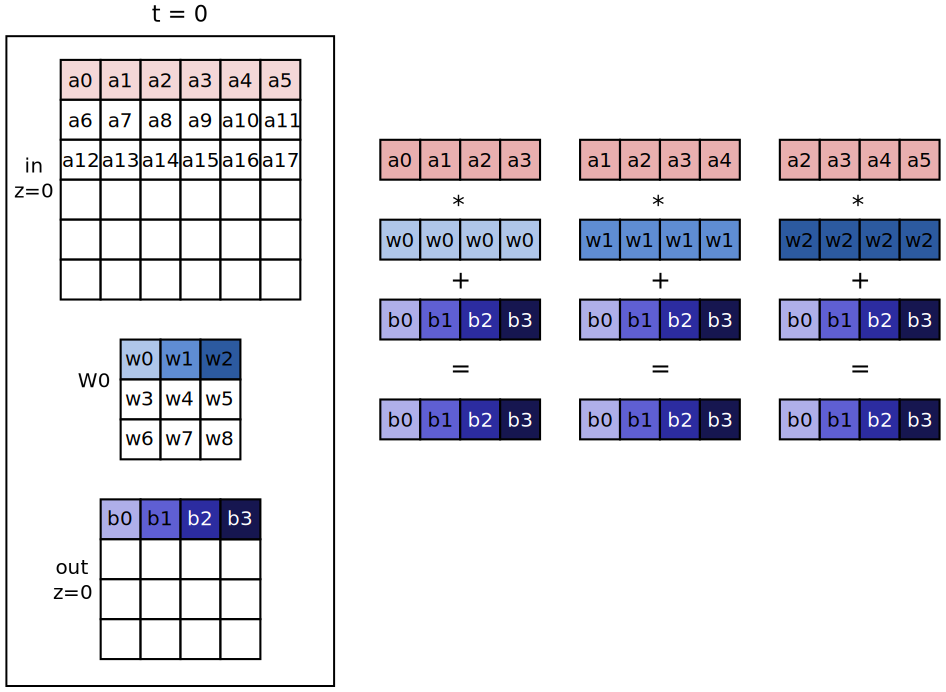
\includegraphics[width=0.5\tw]{fig-tune-vector-convolution-access.svg.pdf}

  \caption{\textbf{Memory Access Pattern for Convolutional Layer --}
    Breakdown of the vector operations required to compute the first row
    of the output in a convolutional layer. Each element in the vector
    corresponds to a separate element in the output. Contiguous elements
    in the input are loaded into a vector register and multiplied with
    the same weight broadcasted to another vector register. The partial
    products are accumulated to the output elements until all weights
    have been applied. Note that the accumulation can be performed in a
    single vector register without intermediate stores.}

  \label{fig-tuning-vectorization-convolution-access}

\end{figure}
